	\begin{figure}[h]
	\centering
		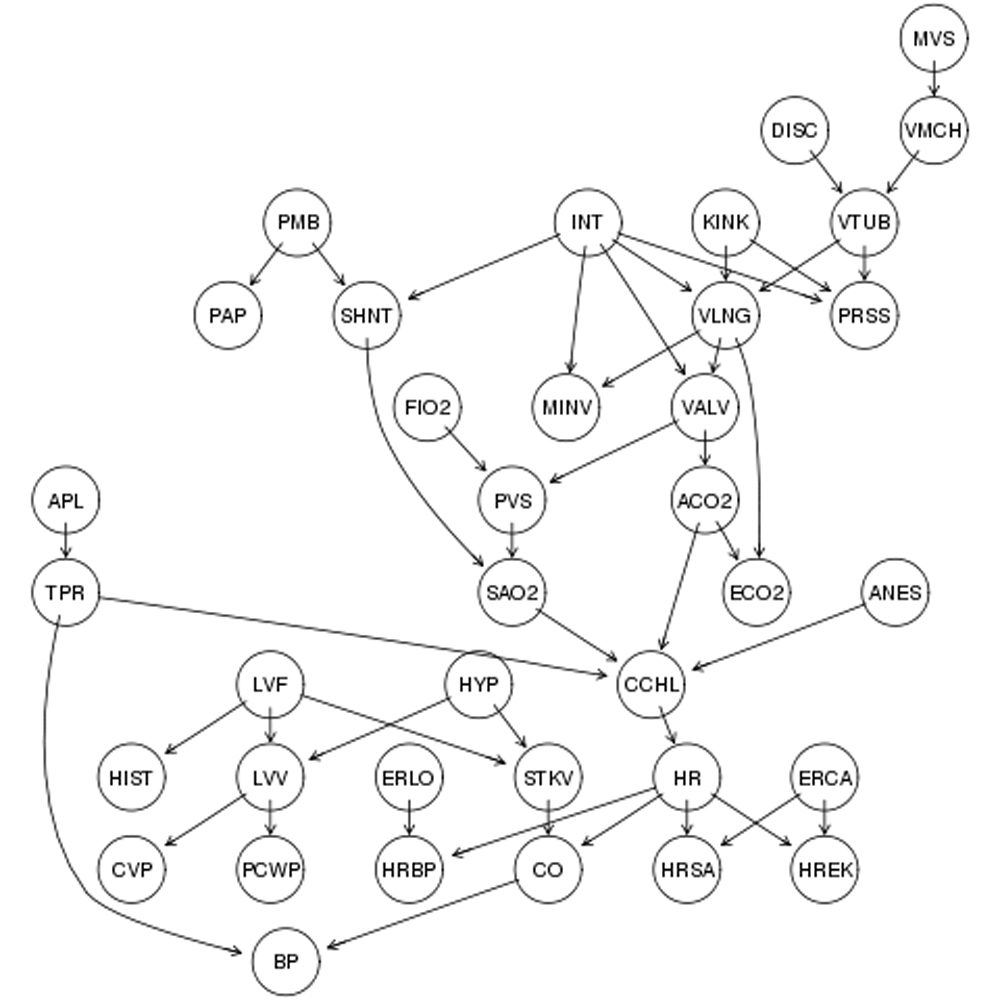
\includegraphics[height=200pt]{Real_Halifinder}
		\caption{Bayesian network model of The HailFinder Weather Forecast System Data Set}
	\end{figure}	

\begin{description}
	\item[Description] Hailfinder is a Bayesian network designed to forecast severe summer hail in northeastern Colorado.

	\item[Number of nodes] 56
	
	\item[Number of arcs] 66
	
	\item[Number of parameters] 2656
\end{description}

Abramson B. \emph{et al.} (1988) motivate this example. Hailfinder is a Bayesian system that combines meteorological data and models with expert judgement, based on both experience and physical understanding, to forecast severe weather in North-eastern Colorado.

% Halifinder
\begin{table}[p]																										
\centering	\caption{Comparison of scores and correct arcs via Hailfinder data set}	\tiny																						
{\tabcolsep=0.01in																										
\begin{tabular}{cc||cc|cc|cc||cc|cc|cc|cc}																										
\hline																										
&	&	\multicolumn{14}{c}{Hailfinder	(Num	of	Nodes	=	56)}\tabularnewline																			
\hline																										
\multicolumn{2}{c||}{Sample	Size}	&	\multicolumn{2}{c|}{1000}	&	\multicolumn{2}{c|}{5000}	&	\multicolumn{2}{c||}{10000}	&	&	&	\multicolumn{2}{c|}{1000}	&	\multicolumn{2}{c|}{5000}	&	\multicolumn{2}{c}{10000}\tabularnewline											
\hline																										
&	&	Sum.	&	Std.Dev.	&	Sum.	&	Std.Dev.	&	Sum.	&	Std.Dev.	&	&	&	Sum.	&	Std.Dev.	&	Sum.	&	Std.Dev.	&	Sum.	&	Std.Dev.\tabularnewline
\hline																										
\hline																										
\multirow{4}{*}{BDe} & HC &	-11006608 & 	381.65 & 	-24975425 & 	256.04 & 	-49602871 & 	297.73 & 	\multirow{4}{*}{C} & HC &	2270 & 	0.96 & 	5301 & 	0.1 & 	5586 & 	0.6\tabularnewline													
& TABU &	-11005176 & 	380.57 & 	-24975425 & 	256.04 & 	-49595842 & 	296.18 & 	& TABU &	2686 & 	1.26 & 	5301 & 	0.1 & 	5473 & 	0.8\tabularnewline													
& MMHC &	-13885378 & 	7417.41 & 	-28286426 & 	1564.45 & 	-56127215 & 	2369.94 & 	& MMHC &	1925 & 	3.09 & 	3247 & 	0.78 & 	3421 & 	1.03\tabularnewline													
& RSMAX2 &	-16586602 & 	3307.55 & 	-30165661 & 	4750.83 & 	-60211607 & 	10590.78 & 	& RSMAX2 &	858 & 	1.19 & 	2513 & 	1.45 & 	2599 & 	1.27\tabularnewline													
\hline																										
\multirow{4}{*}{loglik} & HC &	-10860805 & 	370.7 & 	-24580625 & 	264.37 & 	-49103216 & 	318.52 & 	\multirow{4}{*}{M} & HC &	468 & 	0.69 & 	1299 & 	0.1 & 	974 & 	0.52\tabularnewline													
& TABU &	-10861471 & 	371.47 & 	-24580625 & 	264.37 & 	-49101011 & 	318.75 & 	& TABU &	468 & 	0.69 & 	1299 & 	0.1 & 	975 & 	0.52\tabularnewline													
& MMHC &	-13790813 & 	7449.01 & 	-28061042 & 	1631.98 & 	-55832193 & 	2457.02 & 	& MMHC &	1268 & 	1.56 & 	3350 & 	0.78 & 	3179 & 	1.03\tabularnewline													
& RSMAX2 &	-16508716 & 	3325.33 & 	-30028409 & 	4793.11 & 	-60050894 & 	10637.32 & 	& RSMAX2 &	2949 & 	1.05 & 	4086 & 	1.44 & 	4001 & 	1.27\tabularnewline													
\hline																										
\multirow{4}{*}{AIC} & HC &	-10923175 & 	374.81 & 	-24722989 & 	261.22 & 	-49264998 & 	310.85 & 	\multirow{4}{*}{WO} & HC &	1862 & 	0.9 & 	0 & 	0 & 	40 & 	0.49\tabularnewline													
& TABU &	-10921249 & 	372.87 & 	-24722989 & 	261.22 & 	-49262249 & 	308.38 & 	& TABU &	1446 & 	1.27 & 	0 & 	0 & 	152 & 	0.58\tabularnewline													
& MMHC &	-13816106 & 	7435.45 & 	-28135869 & 	1609.27 & 	-55920440 & 	2432.1 & 	& MMHC &	1407 & 	1.98 & 	3 & 	0.17 & 	0 & 	0\tabularnewline													
& RSMAX2 &	-16527481 & 	3318.41 & 	-30070905 & 	4758.8 & 	-60096326 & 	10600.54 & 	& RSMAX2 &	793 & 	0.71 & 	1 & 	0.1 & 	0 & 	0\tabularnewline													
\hline																										
\multirow{4}{*}{BIC} & HC &	-11148029 & 	416.51 & 	-25186896 & 	253.21 & 	-49848249 & 	291.84 & 	\multirow{4}{*}{WC} & HC &	2714 & 	1.56 & 	1016 & 	0.55 & 	1028 & 	0.75\tabularnewline													
& TABU &	-11136759 & 	427.99 & 	-25186896 & 	253.21 & 	-49843539 & 	288.2 & 	& TABU &	2452 & 	2.25 & 	1016 & 	0.55 & 	1112 & 	1.08\tabularnewline													
& MMHC &	-13907292 & 	7386.76 & 	-28379700 & 	1538.4 & 	-56238585 & 	2345.93 & 	& MMHC &	2368 & 	2.84 & 	1424 & 	2.67 & 	1662 & 	2.16\tabularnewline													
& RSMAX2 &	-16595132 & 	3293.99 & 	-30209383 & 	4647.37 & 	-60260116 & 	10468.63 & 	& RSMAX2 &	2262 & 	1.96 & 	166 & 	1.36 & 	132 & 	1.07\tabularnewline													
\hline																										
\end{tabular}																										
}																										
\end{table}

	\begin{figure}[p]
	\centering
		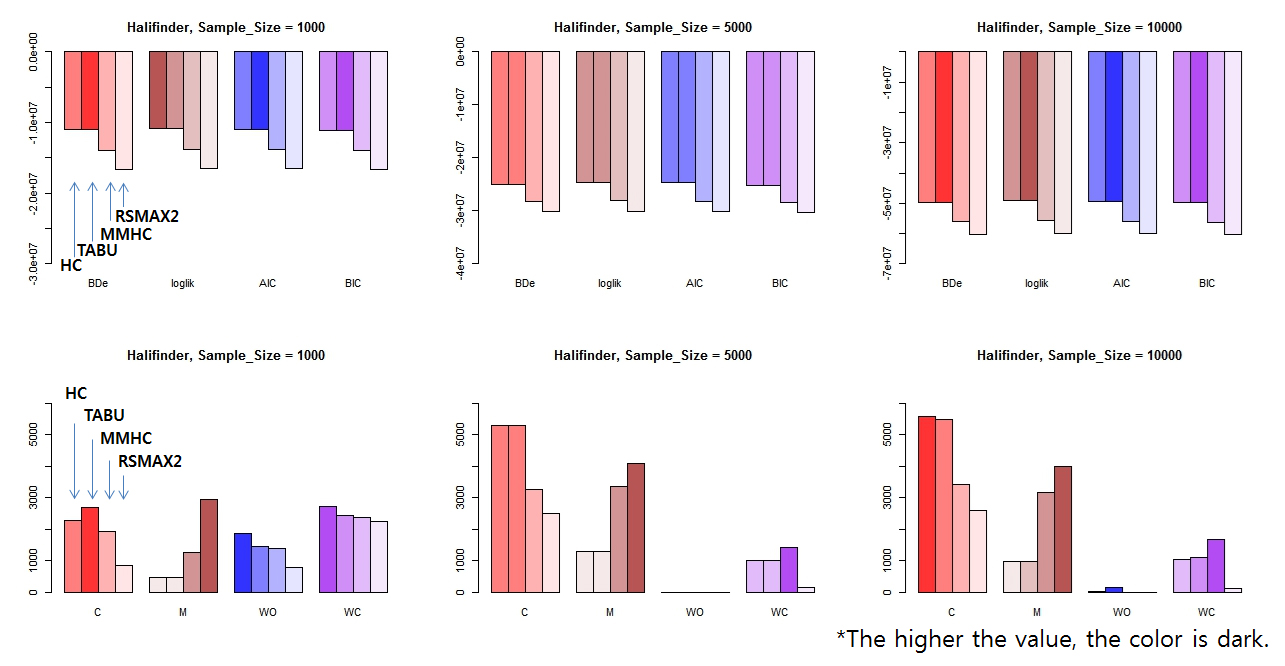
\includegraphics[height=220pt]{Real_4_Halifinder}
		\caption{Comparison of scores and correct arcs via Hailfinder data set}
	\end{figure}	